Zunächst soll im folgenden Kapitel auf die Grundlagen der Deflektometrie und den Stand der Technik eingegangen werden.
Der Begriff \glqq Deflektometrie\grqq ~leitet sich aus dem lateinischen Wort \glqq deflectere\footnote{lat: deflectere: abweichen, abbiegen, ablenken}\grqq ~und dem griechischen Wort \glqq métron\footnote{griech: \textgreek{métron} : Maß, Messung}\grqq ~ab.
Somit bedeutet die Deflektometrie wörtlich übersetzt \glqq Messung der Ablenkung\grqq.
Im wissenschaftlichen Kontext wird die Deflektometrie wie folgt definiert:

\begin{Definition}{Deflektometrie}{def:deflektometrie}
	Die \textit{Deflektometrie} bezeichnet allgemein alle Methoden zur berührungslosen optischen Erfassung von Gestaltinformationen spiegelnder Oberflächen durch automatische Auswertung von Spiegelbildern bekannter Szenen. \cite{fraunhofer}
\end{Definition}

\noindent
Die Übersetzung \glqq Messung der Ablenkung\grqq ~bezieht sich dabei auf das gemessene Spiegelbild der bekannten Szene.
Die Szene wird dabei über eine Oberfläche abgelenkt und schließlich durch einen Sensor als Spiegelbild aufgenommen.
Aus dem Zusammenhang zwischen der Szene und dem Spiegelbild können damit Gestaltinformationen über die spiegelnde Oberfläche berechnet werden.

\begin{figure}[H]
	\centering
	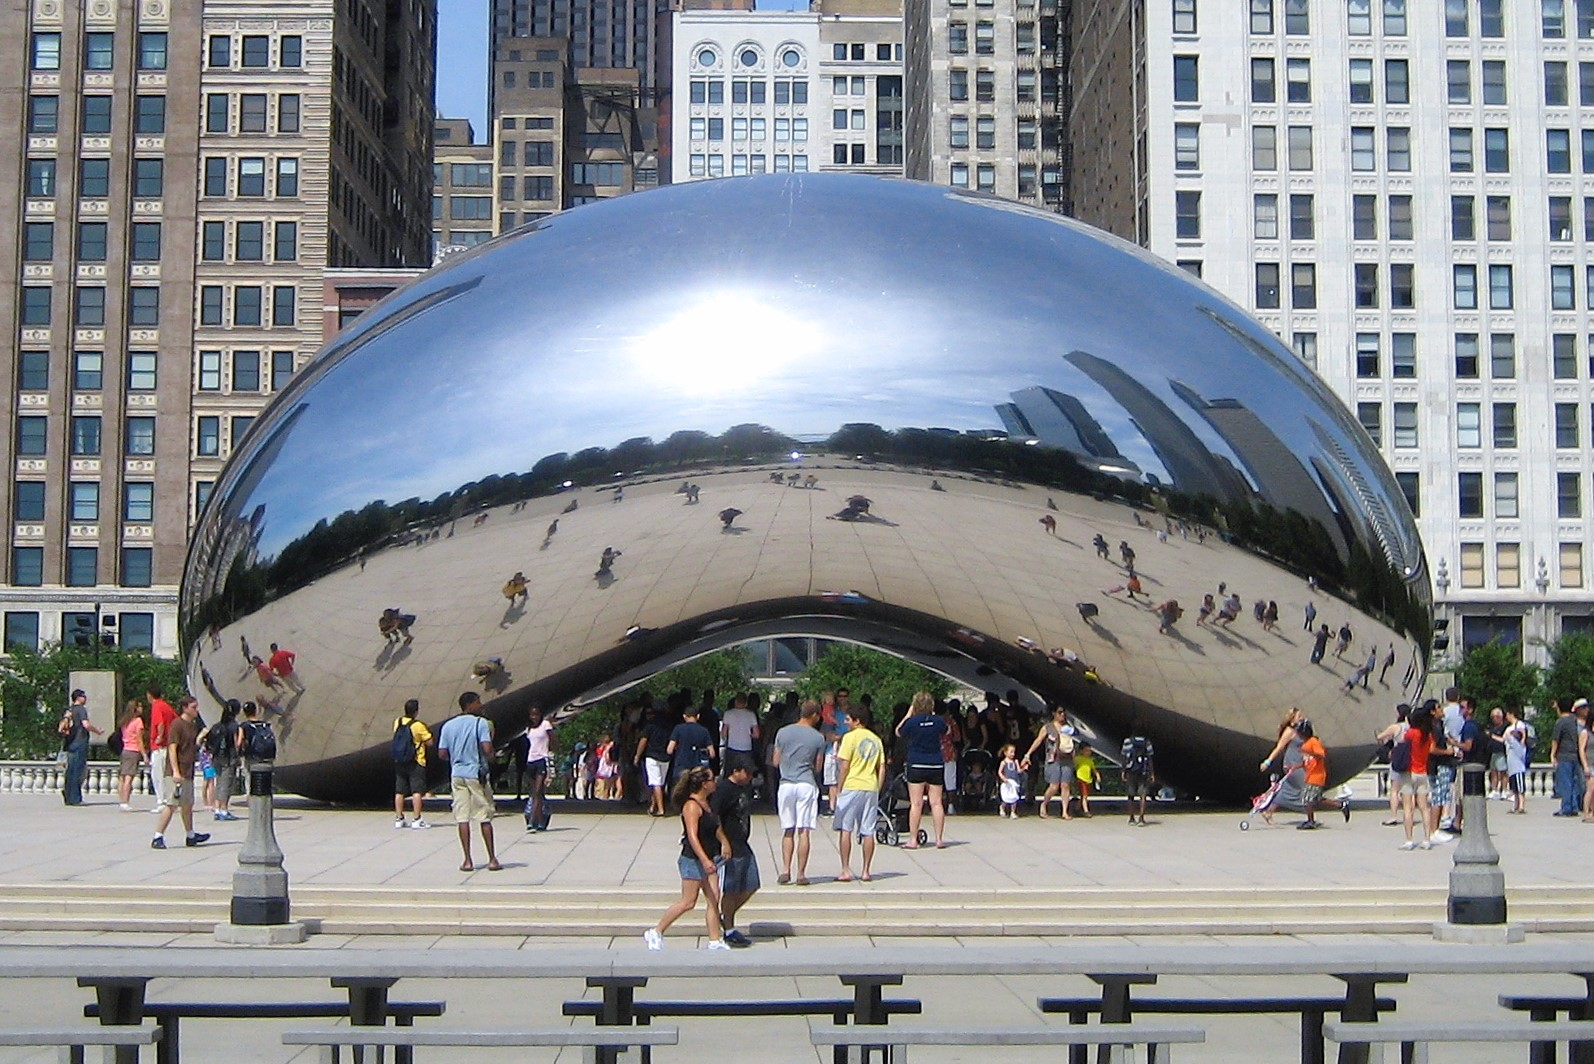
\includegraphics[width=0.55\textwidth]{02_grundlagenZurDeflektometrie/figures/cloud-gate-chicago}
	\caption[Cloud Gate Chicaog - The Bean]{Cloud Gate Chicago - The Bean \cite{cloudGateChicago}}
	\label{img:cloudGateChicago}
\end{figure}

\noindent
In Abbildung \ref{img:cloudGateChicago} erkennt man eine spiegelnde Skulptur, dessen Oberfläche ausschließlich durch die Umgebung und die Spiegelung definiert ist.
Dabei ist es für das menschliche Gehirn zunächst nicht schwierig die Oberflächenform zu interpretieren.
Das liegt an der Betrachtung der Kontextinformation.
Man erkennt z. B. über die Gebäude im Hintergrund die Form der Skulptur.
Zusätzlich mit der Spiegelung der Szene kann man die Krümmung der Oberfläche deuten.
Wenn man den Hintergrund ausblendet, erkennt man die Schwierigkeit der Thematik (siehe Abbildung \ref{img:cloudGateMitAusschnitt}).

\begin{figure}[H]
	\centering
	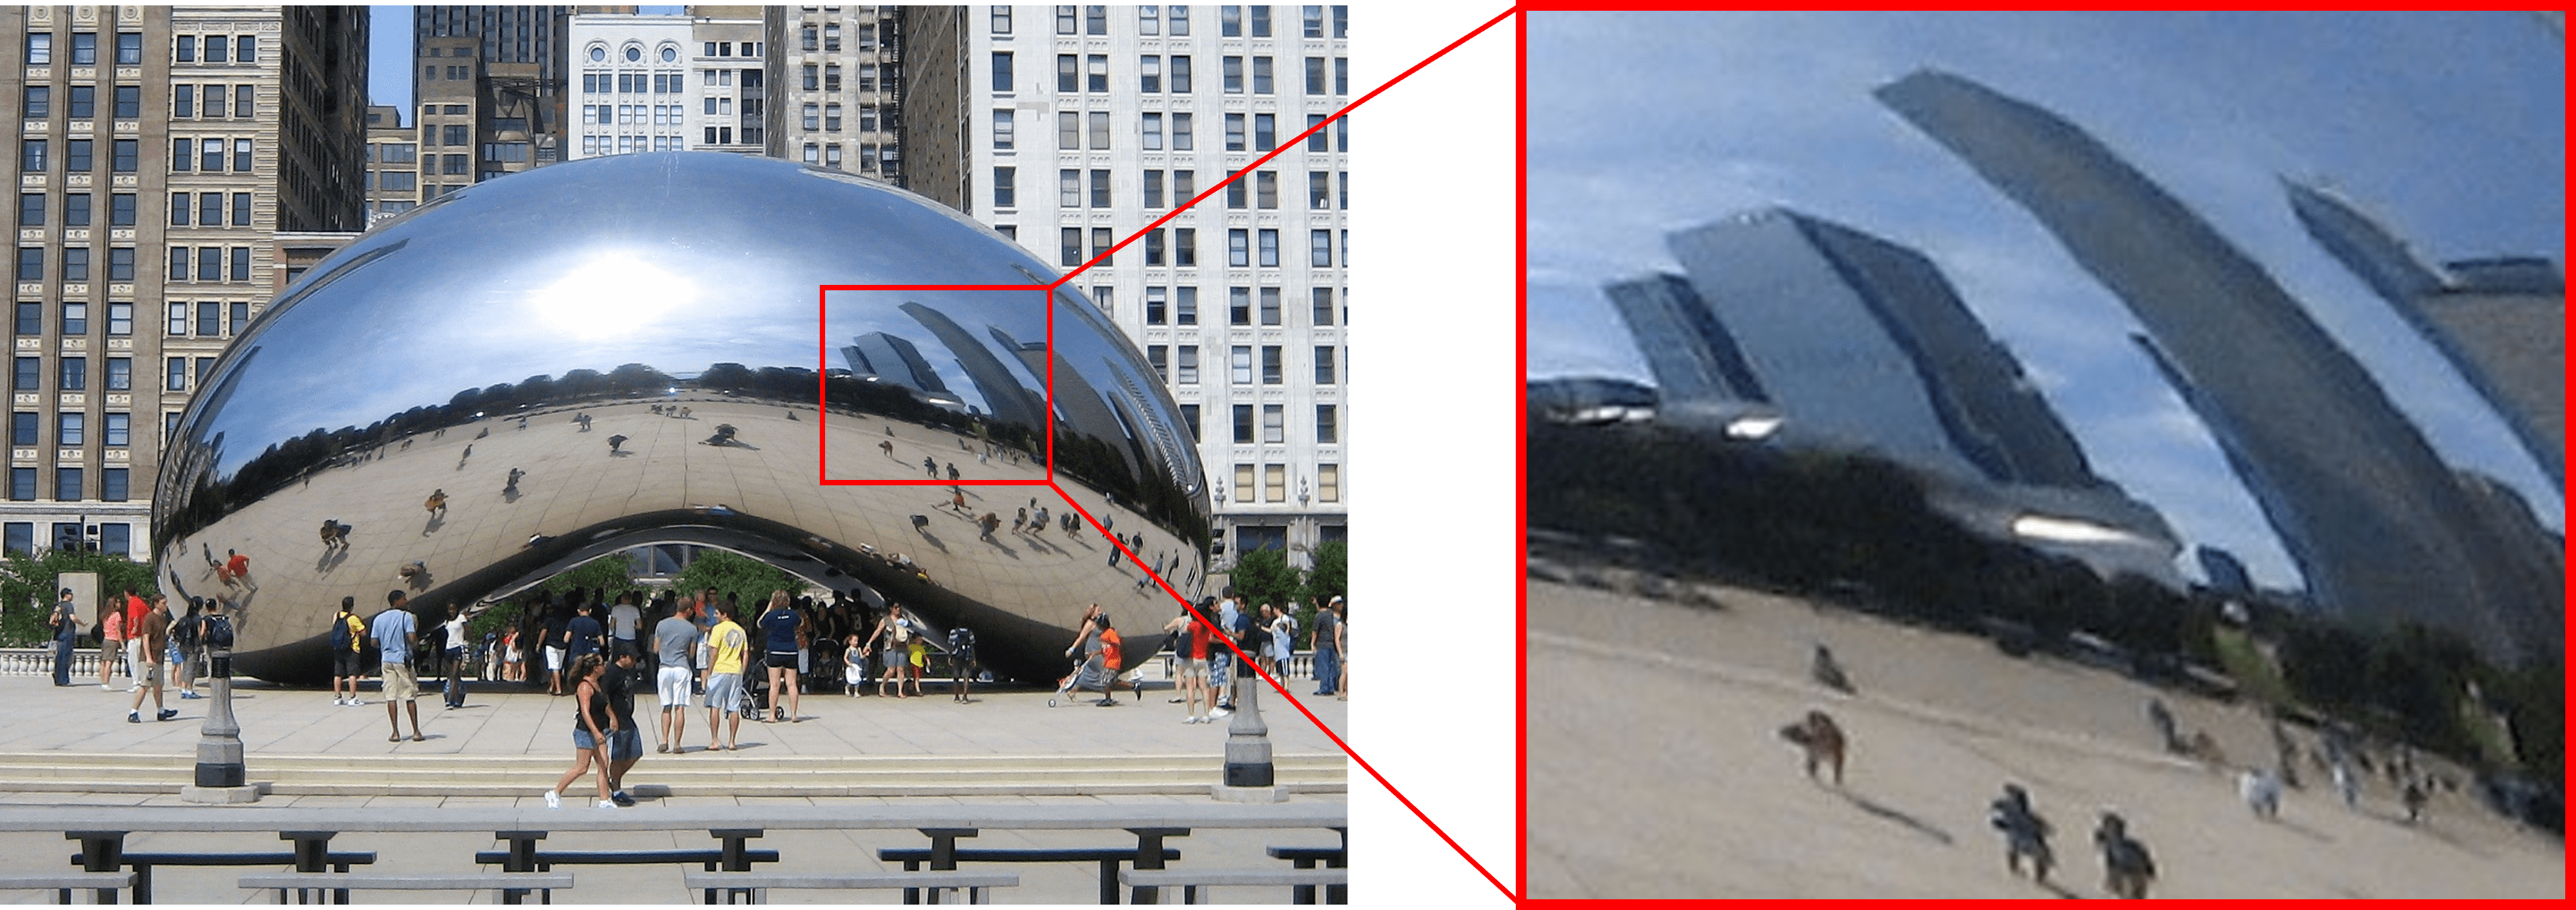
\includegraphics[width=\textwidth]{02_grundlagenZurDeflektometrie/figures/cloudGateMitAusschnitt}
	\caption[Cloud Gate mit Ausschnitt]{Cloud Gate mit Ausschnitt. \textit{in Anlehnung an} \cite{cloudGateChicago}}
	\label{img:cloudGateMitAusschnitt}
\end{figure}

\noindent
Alleine aus dem rechten Ausschnitt von Abbildung \ref{img:cloudGateMitAusschnitt} ist es schon schwieriger zu beurteilen, wie die Skulptur geformt sein könnte.
Zieht man nun Vorwissen über die gespiegelte Szene hinzu, wie z. B. das Wissen über senkrecht stehende Gebäude in Chicago, kann man Aussagen zur Gestalt der lokalen Oberfläche treffen.
Die Schwierigkeit für die automatische Auswertung ist dabei eine eindeutige Zuordnung zwischen der Szene und dem Spiegelbild aufzustellen.
Diese und ähnliche Aufgaben, in denen Spiegelbilder analysiert werden, fallen in das Themengebiet der Deflektometrie.

\p
Die Definition \ref{def:deflektometrie} öffnet ein großes Feld für verschiedene Verfahren und Anwendungen.
Die Verfahren der Deflektometrie sind auch heute noch Themen für viele Forschungsarbeiten.
Im Folgenden soll dabei auf den Stand der Technik der Deflektometrie eingegangen werden.

%Rekonstruktion von spiegelnden Oberflächen
{
	\FloatBarrier
    \section{Rekonstruktion von spiegelnden Oberflächen}
    \label{sub:rekonstruktion}
    Das Hauptforschungsgebiet der gegenwärtigen Deflektometrie die Generierung von dreidimensionalen Modellen von spiegelnden Objektoberflächen ist.
Der Aufbau eines solchen Anwendungsfalls sieht eine Beleuchtungseinheit (z. B. einen Bildschirm), ein Sensor (z. B. eine Kamera) und ein zu untersuchendes Objekt vor.

\begin{figure}[H]
	\centering
	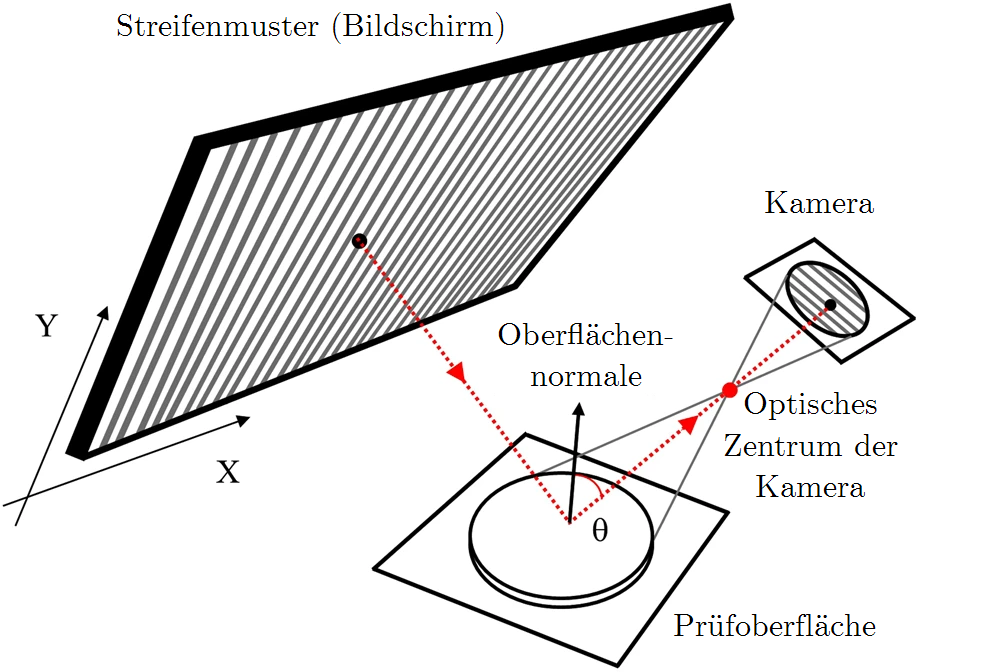
\includegraphics[width=0.7\textwidth]{02_grundlagenZurDeflektometrie/rekonstruktion/figures/nature-articel-nr1}
	\caption[Aufbau einer Deflektometrie-Prüfstation]{Aufbau einer Deflektometrie-Prüfstation. \textit{in Anlehnung an} \cite{aufbau}}
	\label{img:aufbau}
\end{figure}

\noindent
Wie in Abbildung \ref{img:aufbau} angedeutet, wird ein Muster als bekannte Szene auf ein Prüfobjekt projiziert und anschließend von einer Kamera aufgenommen.
Das grundlegende Prinzip basiert darauf, dass jeder durch die Kamera aufgenommene Punkt des Objekts dem richtigen Punkt auf dem Bildschirm zugeordnet wird.
Dabei ordnet man jedem Pixel des projizierten Musters sein zugehöriges Pixel des erzeugten Musters auf dem Bildschirm zu.
Durch diese Zuordnung von Kamera- und Bildschirmpunkten lassen sich Neigungsinformationen der Oberfläche berechnen.
Dies kann durch Strahlenverfolgungen erreicht werden.
In Abbildung \ref{img:aufbau} lässt sich das über die in Rot eingezeichneten Vektoren erkennen.
Wie bereits erwähnt, liegt die Schwierigkeit in der eindeutigen Zuordnung zwischen der Szene und dem Spiegelbild.
Hierfür gibt es verschiedene Ansätze dies zu erreichen.
Grundlegend ist dabei die Kodierung der Objektoberfläche, damit diese durch die Kamera aufgenommen werden kann.
Die Kamera digitalisiert dann die kodierte Oberfläche zu einem oder mehreren Bildern.
Unter Berücksichtigung der Kodierung können die Bilder durch einen entsprechenden Software-Algorithmus dekodiert werden und man erhält damit die Zuordnung zwischen der Szene und dem Spiegelbild (siehe Abbildung \ref{tikz:abbKodierungUndDekodierung}).
%
% Abbildung: Kodierung und Dekodierung
{
	\begin{figure}[H]
		\centering
		\begin{adjustbox}{width=\textwidth}
	\begin{tikzpicture}
	[
		rectnode/.style={rectangle, draw=red!60, fill=red!5, very thick, minimum width={3cm}, font=\small, rounded corners},
		ellipsenode/.style={ellipse, draw=green!60, fill=green!5, very thick, minimum width={3cm}, font=\small},
		calloutnode/.style={rectangle callout, draw=RoyalPurple, fill=RoyalPurple!5, text=RoyalPurple, font=\footnotesize, rounded corners},
	]

		\node[ellipsenode] (source) {Quelle};
		\node[rectnode] (encoder) [right=of source] {Kodierung};
		\node[rectnode] (channel) [below right=of encoder] {Digitalisierung};
		\node[rectnode] (decoder) [below left=of channel] {Dekodierung};
		\node[ellipsenode] (drain) [left=of decoder]{Ergebnis};		
		
		\draw[->] (source.east) -- (encoder.west);
		\draw[->] (encoder.east) -| (channel.north);
		\draw[->] (channel.south) |- (decoder.east);
		\draw[->] (decoder.west) -- (drain.east);
		
		\node[right=of channel, font=\small, align=center] (noise) {Rauschen,\\ Unschärfe};
		\draw[->] (noise.west) -- (channel.east);
		
		\node[calloutnode] (surface) [callout absolute pointer=(source.north), above=of source.east, anchor=east] {Objektoberfläche};
		\node[calloutnode] (illumination) [callout absolute pointer=(encoder.north), above=of encoder.east, anchor=east] {Beleuchtung};
		\node[calloutnode] (camera) [callout absolute pointer=(channel.30), above=of channel.east, anchor=east] {Kamera};
		\node[calloutnode] (software) [callout absolute pointer=(decoder.north), above=of decoder.east, anchor=east] {Algorithmus};
		\node[calloutnode] (result) [callout absolute pointer=(drain.north), above=of drain.east, anchor=east] {Zuordnung};
		
	\end{tikzpicture}
\end{adjustbox}
\caption[Kodierung und Dekodierung der Objektoberfläche]{Kodierung und Dekodierung der Objektoberfläche.}
		\label{tikz:abbKodierungUndDekodierung}
	\end{figure}
}

\noindent
Die Art, wie man die Informationen in den digitalen Kanal überträgt ist entscheidend für eine gute Zuordnung.
Aus dem Grund werden sich einige Gedanken über die Kodierung der Objektoberfläche gemacht.
Auf eine Auswahl von Möglichkeiten soll im Folgenden eingegangen werden.
%
% Phasenkodierung
{
	\FloatBarrier
    \subsection{Phasenkodierung}
    \label{sub:phasenKodierung}
    Die am weitest eingesetzte Kodiermethode in dem Kontext der Deflektometrie ist die Phasenkodierung.
Diese Verfahren werden in dem Themengebiet der \glqq Phasenmessende Deflektometrie\grqq ~beschrieben.
Dabei verwendet man Streifenmuster, die entlang der Ausbreitung der Streifen den Grauwerteverlauf einer Sinus-Funktion annehmen.
Solche Muster nennt man auch sinusoidale Streifenmuster.
Die Szene bzw. der Monitor wird dabei über die Phase der Sinus-Funktion kodiert.
Das heißt, jeder Punkt auf einem Monitor, angegeben durch eine $x$- und eine $y$-Koordinate, wird durch eine Phase $\phi_x$ in $x$-Richtung und eine Phase $\phi_y$ in $y$-Richtung kodiert.
Verwendet man Streifenmuster, stellt man die Kodierung in zwei Bildern dar.
Das erste Bild kodiert die Spaltenpositionen durch die Phasen $\phi_x$ und das zweite Bild kodiert die Zeilenpositionen $\phi_y$ (siehe Abbildung \ref{tikz:abbSinusoidaleStreifenmuster}).

\begin{figure}[H]
	\centering
		\begin{adjustbox}{width=\textwidth}
	\begin{tikzpicture}[every node/.style={inner sep=0,outer sep=0}]
	
		\node [anchor=north east] (imgSpalten) at (-0.03\textwidth,0) {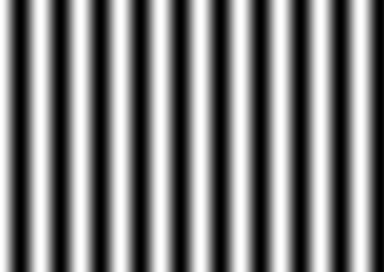
\includegraphics[frame,width=.47\textwidth]{02_grundlagenZurDeflektometrie/rekonstruktion/phasenKodierung/figures/sinusoidalesXMuster}};
		\node [below=0.2cm of imgSpalten, align = center] {Sinusoidales Muster zur Kodierung \\ der Spalten};
		\node [anchor=north west] (imgZeilen) at (0.03\textwidth,0) {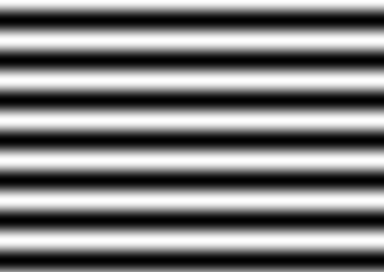
\includegraphics[frame,width=.47\textwidth]{02_grundlagenZurDeflektometrie/rekonstruktion/phasenKodierung/figures/sinusoidalesYMuster}};
		\node [below=0.2cm of imgZeilen, align = center] {Sinusoidales Muster zur Kodierung \\ der Zeilen};
		
	\end{tikzpicture}
\end{adjustbox}
\caption[Sinusoidale Streifenmuster]{Sinusoidale Streifenmuster zur Kodierung der Szene durch die Phasen $\left(\phi_x,\phi_y\right)$.}
		\label{tikz:abbSinusoidaleStreifenmuster}
\end{figure}

\noindent
Der Vorteil ist dabei die Kodierung durch die Grauwerte, die unabhängig von benachbarten Positionen dekodiert werden können.
Zur Dekodierung müssen aus den Grauwerten zunächst die Phasen bestimmt werden.
Dies funktioniert über ein sogenanntes Phasenschiebeverfahren \cite{carre}, bei dem weitere Bildaufnahmen mit Phasenverschiebungen der Sinus-Funktion vorgenommen werden.
Durch die Periodizität der Sinus-Funktion sind die bestimmten Phasen zunächst noch relativ zu den einzelnen Perioden angegeben.
In einem weiteren Schritt muss eine sogenannte Phasenentfaltung bzw. \glqq Unwrapping\grqq ~durchgeführt werden (siehe auch Definition \ref{def:phasenentfaltung}), damit die absoluten Phasen $\left(\phi_x,\phi_y\right)$ bestimmt werden.
Die Dekodierung über das \glqq Unwrapping\grqq ~erfolgt dabei durch die Verwendung von weiteren sinusoidalen Mustern mit unterschiedlicher Frequenz.
Diese Art der Kodierung erfordert damit mehrere Bilder.
Ein solches Verfahren wird im Kapitel \ref{sec:bestimmungDeflektometrischeRegistrierung} genauer beschrieben.

\p
Es sind damit zunächst mehrere Bildaufnahmen erforderlich.
Da solche Verfahren damit mehr Ressourcen verwenden, fokussieren sich einige Forschungsarbeiten die Anzahl der benötigten Muster zu reduzieren.
Der heutige technische Stand, ermöglicht es bereits, z. B. durch Überlagerung von Mustern und weitere Optimierungen, die Phasendekodierung durch eine einzige Kameraaufnahme umzusetzen(vgl. \cite{waveletPMD}).
}
%
% Frequenzkodierung
{
	\FloatBarrier
    \subsection{Frequenzkodierung}
    \label{sub:frequenzKodierung}
    Als Alternative zur Phasenkodierung kann man die Sinus-Funktion auch nutzen um die Ortskoordinaten des Bildschirms über Frequenzen zu kodieren.
Hierfür eignet sich die Darstellung der Koordinaten in der Polarform.
%
\begin{equation*}
	\left(x,y\right) \mapsto \left(r,\phi\right)
\end{equation*}
%
Wenn man im Folgenden den Radius $r$ einer speziellen Frequenz und die Phase $\phi$ als Phasenverschiebung einer Sinus-Funktion zuweist, erhält man zeitabhängige Muster.
So könnte zum Beispiel durch
%
\begin{equation*}
	f_t \left(r,\phi\right) = 1 + \sin \left(2 \pi r t + \phi \right)
\end{equation*}
%
die Kodierung der Szene in Abhängigkeit der Zeit $t$ angegeben sein.
In Abbildung \ref{tikz:abbFrequenzkodierteMuster} wird eine Kodierung dieser Art zu bestimmten Zeitpunkten abgebildet.
%
\begin{figure}[H]
	\centering
	\begin{adjustbox}{width=\textwidth}
	\begin{tikzpicture}[every node/.style={inner sep=0,outer sep=0}]
	
		\node [anchor=north east] (freq0) at (-0.03\textwidth,0) {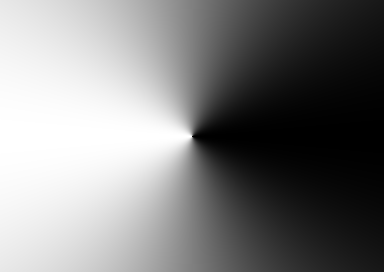
\includegraphics[frame,width=.47\textwidth]{02_grundlagenZurDeflektometrie/rekonstruktion/frequenzKodierung/figures/frequenzKodiertT0}};
		\node [below=0.2cm of freq0] (cap0) {Muster zum Zeitpunkt $t = 0$};
		\node [anchor=north west] (freq1) at (0.03\textwidth,0) {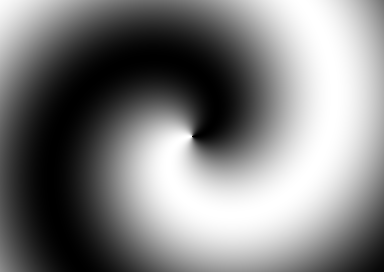
\includegraphics[frame,width=.47\textwidth]{02_grundlagenZurDeflektometrie/rekonstruktion/frequenzKodierung/figures/frequenzKodiertT1}};
		\node [below=0.2cm of freq1] (cap1) {Muster zum Zeitpunkt $t = 1$};
		
		\node [below=1cm of freq0.south east, anchor=north east] (freq4) {
\includegraphics[frame,width=.47\textwidth]{02_grundlagenZurDeflektometrie/rekonstruktion/frequenzKodierung/figures/frequenzKodiertT4}};
		\node [below=0.2cm of freq4] {Muster zum Zeitpunkt $t = 4$};
		\node [below=1cm of freq1.south west, anchor=north west] (freq10) {
\includegraphics[frame,width=.47\textwidth]{02_grundlagenZurDeflektometrie/rekonstruktion/frequenzKodierung/figures/frequenzKodiertT10}};
		\node [below=0.2cm of freq10] {Muster zum Zeitpunkt $t = 10$};
		
	\end{tikzpicture}
\end{adjustbox}
\caption[Muster der Frequenzkodierung]{Muster der Frequenzkodierung der Szene zu festen Zeitpunkten $t$.}
	\label{tikz:abbFrequenzkodierteMuster}
\end{figure}
%
\noindent
Zur Dekodierung muss hier über eine gewisse Zeit die Frequenz der einzelnen Bildpunkte gemessen werden.
Zusätzlich muss der Phasenwinkel bestimmt werden.
Dafür kann ein ähnliches Verfahren wie auch bei der Bestimmung der Phase im vorhergehenden Abschnitt \ref{sub:phasenKodierung} eingesetzt werden.
Zur Optimierung des Rechenaufwands ist es auch möglich, jeder Ortskoordinate eine eigene Frequenz zuzuweisen, damit man sich die Bestimmung der Phase sparen kann.

\p
Da in diesem Kodierverfahren nicht mehr die Grauwerte des Bildes selbst den Ort kodieren, ist es unempfindlich gegenüber Nichtlinearitäten in den Anzeige- oder Aufnahmefarben.
Außerdem lassen sich mehrere Signale überlagern und genau durch die Frequenz trennen.
Ein großer Nachteil im Vergleich zur Phasenkodierung ist allerdings die lange Messzeit der Frequenz \cite{jenaerOK}.
}
%
% Stochastische Kodierung
{
	\FloatBarrier
    \subsection{Stochastische Kodierung}
    \label{sub:stochastischeKodierung}
    Die stochastische Kodierung nutzt ein zufällig generiertes Muster als Szene.
Geeignet für dieses Verfahren sind sogenannte \glqq Specklemuster\grqq ~\cite{specklePattern}.
Es handelt sich dabei um bandbegrenzte Muster mit zufällig verteilten Grauwerten.
Aufgrund der Unschärfe und dem Rauschen, welche in der Aufnahme durch eine Kamera einfließen, ist die Bandbegrenztheit notwendig um eine Dekodierung zu ermöglichen.
Abbildung \ref{img:speckleMuster} zeigt ein solches Muster.
%
\begin{figure}[H]
	\centering
	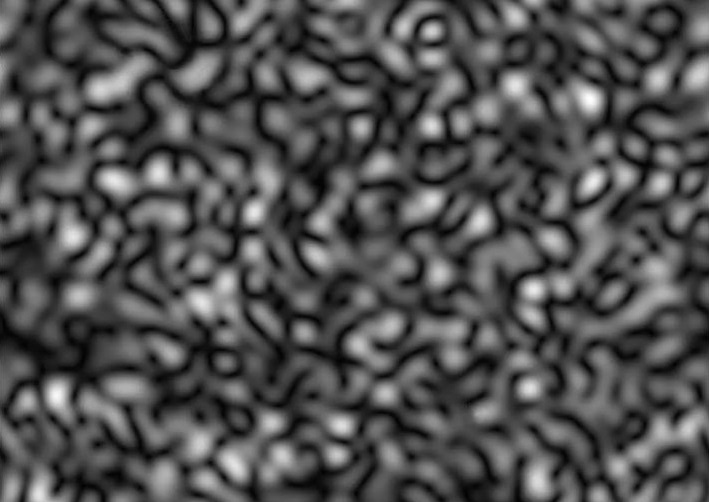
\includegraphics[frame,width=0.5\textwidth]{02_grundlagenZurDeflektometrie/rekonstruktion/stochastischeKodierung/figures/speckleMuster}
	\caption[Specklemuster]{Specklemuster.}
	\label{img:speckleMuster}
\end{figure}
%
Das Prinzip sieht drei Aufnahmen unter Beobachtung des erzeugten Specklemusters vor.
Zunächst die Aufnahme des 
}
%
\p
Ist erstmal die Zuordnung durch die Dekodierung erfolgt, kann man weitergehend die Oberfläche rekonstruieren.
Nimmt man zusätzlich die Informationen über den Systemaufbau hinzu bzw. führt eine Systemkalibrierung durch, kann aus der Zuordnung von Kamera- und Bildschirmpunkten der Reflexionswinkel $\theta$ aus Abbildung \ref{img:aufbau} berechnet werden.
Da bei einer Reflexion die Lichtstrahlen genau an der Oberflächennormalen gespiegelt werden, lässt sich dann in einem weiteren Schritt die Oberflächennormale in diesem Punkt bestimmen.
Führt man dies für jeden Punkt im Kamerabild durch, erhält man daraus die Neigungsinformationen des zu prüfenden Objektes in der Form eines Normalenfelds.

\p
Schließlich ist es möglich, aus diesem Normalenfeld räumliche Information der Oberfläche zu berechnen.
Dafür kann man zunächst aus den Normalenvektoren die zugehörigen Tangentialebenen berechnen, die über je zwei Richtungsvektoren definiert sind.
Diese Richtungsvektoren bilden die Tangentialfelder des Prüfobjekts.
Man kann über eine Integration der Tangentialfelder in ausgewählte Richtungen Kurven bestimmen, die in der Oberfläche des Objekts liegen.
Durch diese Integration erhält man einen Höhenzusammen\-hang der Oberflächenpunkte.
Wenn zusätzlich ein Oberflächenpunkt gegeben ist, kann man die dreidimensionalen Positionen der Oberflächenpunkte im Raum angeben \cite{kit_werling}.
}

%Qualitative Sichtprüfung
{
	\FloatBarrier
    \section{Qualitative Sichtprüfung}
    \label{sub:qualitativeSichtpruefung}
    Der Bereich der qualitativen Sichtprüfung hat grundlegend die Aufgabe, spiegelnde Oberflächen nach bestimmten Kriterien in gut und fehlerhaft zu unterteilen.
Die Aufbauten für solche Verfahren sehen in der Regel ähnlich aus wie auch in Abbildung \ref{img:aufbau}.
Zur Analyse dieser spiegelnden Oberflächen ist es nicht unbedingt nötig, ein dreidimensionales Oberflächenmodell zu erzeugen.
Ein wesentlicher Unterschied ist deshalb, dass die Informationen über den Systemaufbau nicht zwingend notwendig für Berechnungen sind.
Um eine möglichst allgemein einsetzbare Lösung zu entwickeln, ist dies ein essenzieller Vorteil.
Die Vorgehensweise bei diesen Verfahren basiert in den meisten Fällen darauf, die Abweichungen der Oberflächenstruktur zu einem Referenzobjekt zu bewerten.
Abhängig von den einzelnen Oberflächenmerkmalen können verschiedene Muster und Strategien zur Auswertung eingesetzt werden.

\p
In seiner Dissertation \glqq Deflektometrie zur automatischen Sichtprüfung und Rekonstruktion spiegelnder Oberflächen\grqq ~\cite{kit_werling} listet Stefan Bruno Werling vom Karlsruher Institut für Technologie einige Auswertungsmöglichkeiten auf.
Daraus sind die Folgenden eine Auswahl seiner Strategien:

\begin{itemize}
	\item Untersucht man auf der Oberfläche eines Objekts ein sinusförmiges Streifenmuster, dann können im Frequenzraum Abweichungen des Musters von einem \glqq Idealmuster\grqq ~bzw. Referenzmuster festgestellt werden.
	Dadurch entdeckt man Unterschiede in der Oberflächenkrüm\-mung.
	Die Transformation des Bildes in den Frequenzraum wird durch die Fourier-Transformation erreicht.
	
	\item Nutzt man zur Auswertung ein Schachbrettmuster, so können durch die Wahl eines geeigneten Schwellwerts bestimmte Flächen segmentiert und geometrisch analysiert werden.
	Nach der Analyse sollen Anomalien der geometrischen Merkmale Aussagen über die Krümmung treffen.
	
	\item Besonders kleine Fehler und Defekte der Oberflächenstruktur lassen sich an Hell-Dunkelübergängen gut hervorheben.
	Hierfür kann man einfache Streifenmuster analysieren, wie es in Abbildung \ref{img:scratch} gezeigt ist.
\end{itemize}

\begin{figure}[H]
	\centering
	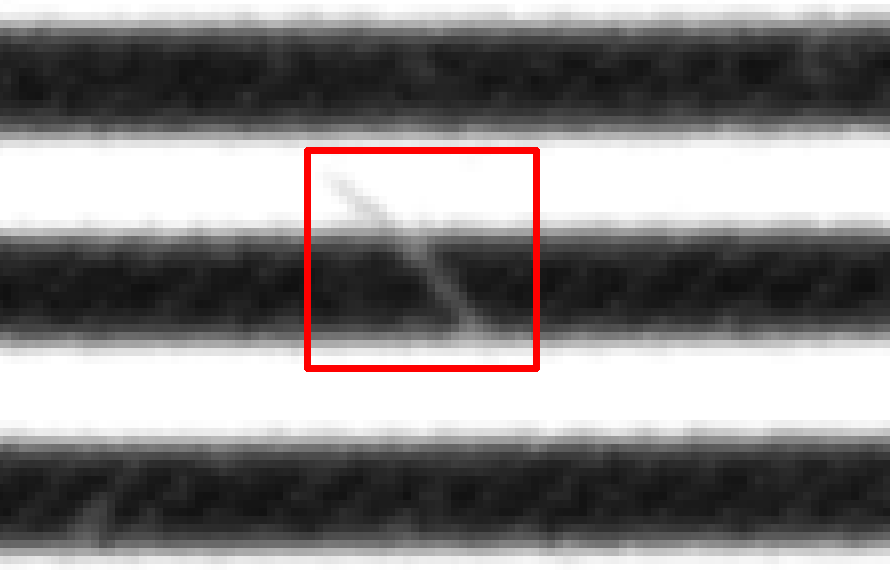
\includegraphics[width=0.5\textwidth]{02_grundlagenZurDeflektometrie/qualitativeSichtpruefung/figures/scratch}
	\caption[Kratzer an Hell-Dunkel-Übergang eines Streifenmusters]{Kratzer an Hell-Dunkel-Übergang eines Streifenmusters}
	\label{img:scratch}
\end{figure}

\noindent
Durch die Variabilität der Deflektometrie und der offenen Definition der qualitativen Sichtprüfung lassen sich z. B. durch Veränderung bestimmter Muster zahlreiche verschiedene Verfahren aufstellen, um eine Objektoberfläche zu analysieren.
Aus dem Grund kann keine allgemeine Funktionsweise von deflektometrischen Verfahren für die qualitative Sichtprüfung beschrieben werden.
%Stattdessen wird im Rahmen dieses Projekts auf ein bestimmtes ausgewähltes Verfahren genauer eingegangen, dass für die konkreten Anwendungsfälle aus Kapitel \ref{sec:projektthema} Ergebnisse liefern konnte.
}